\documentclass[parskip]{scrartcl}
\usepackage[utf8]{inputenc}
\usepackage[ngerman]{babel}
\usepackage[round]{natbib}
\usepackage{graphicx}
\usepackage[automark]{scrpage2}
\usepackage{setspace}
\usepackage{csquotes}
\usepackage{amsmath}
\usepackage[usenames,dvipsnames]{color}
\usepackage{listings}
\usepackage{url}
\usepackage{setspace}
\usepackage[colorlinks=false, pdfborder={0 0 0}]{hyperref}
\lstset {
  language=java,
  basicstyle={\footnotesize\ttfamily},
  numbers=none,
  aboveskip=5mm,
  belowskip=5mm,
  showstringspaces=false,
  columns=flexible,
  keywordstyle=\color{red},
  commentstyle=\color{red},
  stringstyle=\color{magenta},
  frame=single,
  breaklines=true,
  breakatwhitespace=true,
  tabsize=4,
  morekeywords={ }% <-- adding custom keywords
}

\begin{document}
\subject{Projektdokumentation im Modul Smartcard}
\title{Patientendateninformationskarte im medizinischen Sektor}
\author{Robert Kupferschmied B.Sc., Roy Meissner B.Sc.,\\Sebastian Krause B.Sc.}
\date{\today}

\maketitle
\onehalfspacing
\section{Anwendungsbeschreibung}
	Die Anwendung wurde zum Zweck entworfen, Mitarbeitern im medizinischem Sektor schnell Daten über die bedürftige Person bzw. dem Patienten zur Verfügung zu stellen. Zu diesem Zweck wurde ein System bestehend aus einer OffCard-Anwendung, die zur Beispielhaften Demonstration des medizinischen Personals da ist, sowie einer OnCard-Anwendung, die verschiedene Daten eines Patienten speichert, entworfen.
	
	Die OffCard-Anwendungen lässt es zu, eine Rolle auszuwählen. Anhand dieser Rolle kann auf verschiedene Funktionalitäten der SmartCard zugegriffen werden, je nachdem welche Rechte die Rolle besitzt. Hauptanwendungszweck der OffCard-Anwendung ist die Anzeige der auf der SmartCard gespeicherten Daten, als auch die Manipulation dieser.
	
	Die OnCard-Anwendung speichert Patientenbezogene Daten, wie dessen Blutgruppe, dessen ID, sowie mehrere Listen von Medikamenten. Diese Daten können von den entsprechenden Rollen manipuliert werden.
	
	Um eine Absicherung gegen Angriffe bereit zu stellen, als auch die Rollen untereinander zuverlässig trennen zu können, wird eine Verschlüsselung der übertragenen Daten durchgesetzt.
\section{OffCard}
\section{OnCard}
	Die OnCard-Anwendung bietet eine vollständig definierte Schnittstelle in Form von APDU-Beschreibungen an. Über diese Schnittstelle kann mit den Daten, die auf der Smartcard gespeichert sind, interagiert werden.
	
	Die Smartcard enthält in der folgenden Auflistung enthaltene Daten:
	
	\begin{itemize}
		\item eine Patienten-ID
		\item die Patientenblutgruppe
		\item eine Liste nicht verträglicher Medikamente
		\item eine List regelmäßig einzunehmender Medikamente mit Dosierungsinformationen, bestehend aus Medikamente-ID(s), Menge(n) und Zeitpunkt(en)
	\end{itemize}
	
	Die Patienten-ID wird zur Installation des Applets auf der Karte fest ein kodiert. Die ID ist eine Zahl vom Typ long, die auf der Smartcard in Form von 8 Bytes abgespeichert wird. Die ID kann über die Schnittstelle nur abgerufen, nicht aber verändert werden.
	
	Ein beispielhafter Abruf der Patienten-ID sieht wie folgt aus:
	
	\begin{lstlisting}
		\send 00 08 00 00
		Response:
		00 00 00 00 00 00 00 01 90 00 //Patienten-ID + No-Error-Code
	\end{lstlisting}
	
	Die Blutgruppe des Patienten wird, wie die Patienten-ID, zur Installation des Applets festgelegt. Sie ist als ein Byte codiert und kann anhand einer Kodierungstabelle übersetzt werden. Wie die Patienten-ID ist auch die Blutgruppe nicht manipulierbar.
	
	Ein beispielhafter Abruf der Patienten Blutgruppe sieht wie folgt aus:
	
	\begin{lstlisting}
		\send 00 07 00 00
		Response:
		04 90 00 //Blutgruppe + No-Error-Code
	\end{lstlisting}
	
	Auf der Smartcard wird eine Liste nicht verträglicher Medikamente gespeichert. Diese ist als eine List von jeweils 4 Byte IDs angelegt. Diese IDs können in der OffCard-Anwendung in ein Int umgewandelt und über eine Map dem entsprechenden Medikament zugeordnet werden. Die Smartcard bietet an, die Liste Elementweise auszulesen, neue Medikamente zur Liste hinzuzufügen, als auch aus der Liste zu entfernen.
	
	Ein beispielhaftes Hinzufügen eines Medikaments zur Liste sieht wie folgt aus:
	
	\begin{lstlisting}
		\send 00 02 00 00 04 00 00 42 83 //Add Element with ID 00 00 42 83
		Response:
		Success: 90 00
		Failure: 6A 83
	\end{lstlisting}
	
	Ein beispielhafter Abruf eines Medikaments der Liste sieht wie folgt aus:
	
	\begin{lstlisting}
		\send 00 01 00 00 //Fetch Element 0
		Response:
		Success: 00 00 42 83 90 00 //Drug-ID + No-Error-Code
		Failure: 6A 83
	\end{lstlisting}
	
	Ein beispielhaftes löschen eines Medikaments der Liste sieht wie folgt aus:
		
	\begin{lstlisting}
		\send 00 03 00 00 04 00 00 42 83 //Remove Element with ID 00 00 42 83
		Response:
		Success: 90 00
		Failure: 6A 83
	\end{lstlisting}
	
	Die Liste der regelmäßig einzunehmenden Medikamente ist gleich der Liste nicht verträglicher Medikamente aufgebaut, nur das die Eintragslänge 28 Byte entspricht. Die ersten 4 Byte entsprechen der Medikamenten-ID, die folgenden 24 Byte den Einnahmezeiträumen sowie der Einnahmemenge. Diese Liste kann ebenfalls ausgelesen und manipuliert werden.
	
	Die Kommandos dieser Liste sind analog zur Liste der nicht verträglichen Medikamente definiert.
	
	Intern werden die Liste über eine, eigens für diesen Zweck erstellte, Collection organisiert. Diese bietet ein List-Interface fü das kontrollierte Hinzufügen, Löschen als auch Auslesen der Listenelemente.
\section{Kryptologie}
In diesem Kapitel werden die kryptografischen Methoden des Projektes erklärt. Zum Verschlüsseln der Daten wird ein symmetrisches Verfahren verwendet. Symmetrische Verschlüsselungsverfahren sind sehr effizient und sicher. Leider werden bei symmetrischen Verfahren nur ein Schlüssel zum Ver- und Entschlüsseln verwendet. Deswegen ist der Schlüsselaustausch sehr schwierig. Asymmetrische Verfahren können dieses Problem lösen.
\subsection{Asymmetrische Verschlüsselung - RSA}
Zur asymmetrischen Verschlüsselung stehen auf den Smartcards prinzipiell zwei Algorithmen zur Verfügung. Zum einen der \enquote{elliptic Curve}-Algorithmus und der RSA\footnote{Rivest, Shamir und Adleman}-Algorithmus. Die Sicherheit des RSA-Algorithmus beruht auf dem Problem der Primzahlzerlegung. Das Problem der Primzahlzerlegung ist ein schwieriges Problem, da kein effizienter Algorithmus bekannt ist der das Problem lösen könnte. Weiterhin ist RSA der bekannteste und am weitesten verbreitete Algorithmus zur asymmetrischen Verschlüsselung. Um zu möglichst vielen Systemen kompatibel zu sein, wird der RSA-Algorithmus in diesem Projekt verwendet.\\
Bei asymmetrischen Verschlüsselungsverfahren werden Schlüsselpaare für die Verschlüsselung benutzt. Diese Schlüsselpaare bestehen aus einem Public-Key und einem Private-Key. Der Public-Key kann publiziert werden. Den Private-Key muss man geheim halten.\\
Die Schlüssel setzen sich aus einem Exponenten und einem Modulus. Der Modulus ist eine sehr große Zahl, bei RSA-1024 eine Zahl im Bereich von $ 2^{1024} $ und setzt sich aus zwei Primzahlen zusammen. Der Modulus ist im Public- und Private-Key gleich. Die Exponenten unterscheiden sich allerdings.\\
Zur Ver- und Entschlüsselung werden folgende Funktionen benutzt:  
 $$ G = K^{e}\mod{n} $$
 $$ K = G^{d}\mod{n} $$
 Legende: \\
 G .. Geheimtext\\
 K .. Klartext\\
 e .. öffentlicher Exponent\\
 d .. geheimer Exponent\\
 n .. Modulus\\
Die Schlüssel werden im der Datei \enquote{irgendwas.java} erzeugt. Hier sind diese Zeilen wichtig:
\label{RSAKeyPair}
\begin{lstlisting}
Cipher rsaCipher = Cipher.getInstance(Cipher.ALG_RSA_PKCS1,false);
KeyPair keyPair = new KeyPair(KeyPair.ALG_RSA_CRT, (short)1024);
keyPair.genKeyPair();
RSAPrivateCrtKey rsa_privateKey = (RSAPrivateCrtKey) keyPair.getPrivate();
RSAPublicKey rsa_publicKey = (RSAPublicKey) keyPair.getPublic();
\end{lstlisting}
Die JCOP Shell hat beim erstellen der Schlüssel leider ein paar Fehler. Hier kann beim erzeugen des öffentlichen Schlüssels kein echter öffentlicher Exponent erzeugt werden, stattdessen wird nur eine konstante binäre 17 zurückgegeben.\\
Auf einer echten Karte dürfte dieser Fehler nicht auftreten.\\
Die Verschlüsselung mit asymmetrischen Verfahren ist nicht so effizient, wie die Verschlüsselung mit symmetrischen Verfahren. Deswegen ist es sinnvoll die symmetrische und asymmetrische Verfahren zu kombinieren um die Vorteile aufzuwiegen. Asymmetrische Verfahren werden dazu verwendet um den Schlüssel der symmetrischen Verfahren auszutauschen.

\subsection{Symetrische Verschlüsselung - DES,AES}
Für die symmetrische Verschlüsselung ist nur ein Schlüssel für die Ver- und Entschlüsselung notwendig. Dieser wird von dem Off-Card Programm erzeugt und via RSA-Verschlüsselung an die Karte gesendet. Als Verschlüsselungsalgorithmus wird DES benutzt. Dieser besitzt eine Schlüssellänge von 56-Bit. DES gilt nicht mehr als sicher da die Schlüssellänge zu kurz ist. Normalerweise nutzt man bei der modernen Verschlüsselung AES. Dieser gilt als mathematisch sicher und man kann ihn nur angreifen indem man alle möglichen Schlüssel durchprobiert. AES besitzt einen Schlüsselraum von 128 Bit und kann auf 256 Bit erweitert werden.\\ 
AES wird nicht von der Simulationsumgebung JCOP unterstützt, deswegen muss man DES einsetzen. Im Betrieb mit einer echten Karte sollte man allerdings AES verwenden.\\
Sowohl AES als auch DES verschlüsseln die Daten Blockweise. Deswegen gibt es verschiedene Modi beim Verschlüsseln. Hier kann man folgende Modi einstellen:
\begin{lstlisting}
Cipher.getInstance(Cipher.ALG_DES_ECB_NOPAD,false);
Cipher.getInstance(Cipher.ALG_DES_ECB_PKCS5,false);
\end{lstlisting}
Das Cipher-Objekt spricht den Kryptologie-Prozessor der Smartcard an. Der Algorithmus ist DES. ECB steht für Electronic Code Book, dies ist besonderer Sicherheitsmodus damit ähnliche Daten nicht erkannt werden. NOPAD steht für No Padding, hier können nur Daten verschlüsselt werden deren Länge ein vielfaches der Blocklänge entspricht. Im Modus PKCS5 wird der Klartext um die Fehlenden Bytes 

\section{OpenCard Framework - OCF}
Das OpenCard Framework ist eine Smartcard Middleware. Hiermit kann man mit Smartcards kommunizieren. Das OpenCard Framework ist komplett in Java programmiert und damit Betriebssystemunabhängig.\\
Um mit einer Smartcard kommunizieren zu können muss man zunächst die Verbindung aufbauen. Dafür einfach folgende Methoden ausführen:
\begin{lstlisting}
CardRequest cardRequest = new CardRequest(CardRequest.ANYCARD, null, PassThruCardService.class);
cardRequest.setTimeout(1);
card = SmartCard.waitForCard(cardRequest);
\end{lstlisting}
Nun kann man über die \enquote{card} Variable APDU's an die Smartcard senden. Hierfür muss man folgende Methoden senden:
\begin{lstlisting}
CommandAPDU commandAPDU = new CommandAPDU(instruction.length);
commandAPDU.setLength(instruction.length);
System.arraycopy(instruction, 0, commandAPDU.getBuffer(), 0, instruction.length);
PassThruCardService passThru = (PassThruCardService) card.getCardService(PassThruCardService.class, true);
ResponseAPDU responseAPDU1 = passThru.sendCommandAPDU(commandAPDU);
\end{lstlisting}
Zunächst wird eine APDU angelegt, danach kann man sie mit Bytes beschreiben. Über den Befehl \enquote{sendCommandAPDU} wird die APDU an die Smartcard gesendet und als Rückgabewert wird die empfangene APDU zurückgeben.\\
\section{Schlüsselaustausch mit OCF}
Die Abbildung \ref{fig:KeyExchange} visualisiert den Ablauf.

\begin{figure}[h]
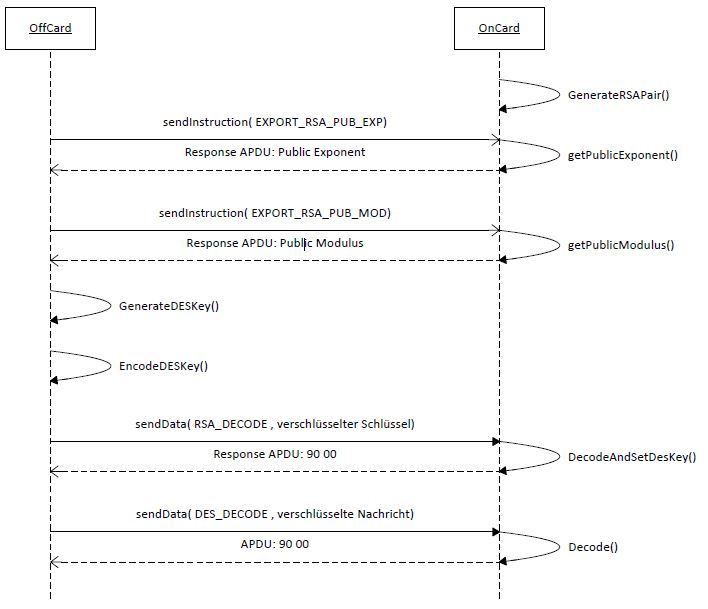
\includegraphics[width=1.2\linewidth]{./KeyExchange}
\caption{Schlüsselaustausch}
\label{fig:KeyExchange}
\end{figure}

\begin{tabular}{|l|l|}
\hline Funktion & befindet sich in Datei \\ 
\hline
\hline sendInstruction( ) & Install.java \\ 
\hline sendData( ) & Install.java \\ 
\hline GenerateRSAPair()  & RSA.java \\ 
\hline getPublicExponent() & RSA.java \\ 
\hline getPublicModulus() & RSA.java \\ 
\hline GenerateDESKey() & Install.java \\ 
\hline EncodeDESKey() & Install.java \\
\hline DecodeAndSetDesKey() & RSA.java \\
\hline Decode() & RSA.java \\
\hline 
\end{tabular} 

Beim installieren der Smartcard-Applikation wird ein RSA Schlüsselpaar erzeugt. Dies geschieht über die in Kapitel \ref{RSAKeyPair}. Über die definierten Kommando APDU's \\\enquote{EXPORT\_RSA\_PUB\_EXP} und \enquote{EXPORT\_RSA\_PUB\_MOD} kann man sich den Public-Key der Karte ausgeben lassen. Der Exponent und Modulus könne in Java durch die BigInteger-Klasse zu einem RSA-Key zusammengesetzt werden. Dann wird der DES-Key von der OffCard-Anwendung erzeugt. Diesen kann man nun mit RSA verschlüsseln und an die Karte senden. In der Karte wird der Schlüssl mit dem privaten RSA-Schlüssel entschlüsselt. Nun ist der DES-Schlüssel ausgetauscht und man kann effizient symmetrisch verschlüsseln. Um mit DES Ver- und Entschlüsseln zu können ist es wichtig die Richtigen Modi einzustellen. Die virtuelle Karte von JCOP unterstützt nicht alle Modi. Wenn man den CBC\footnote{Cipher Block Chaining}-Modus einstellt entschlüsselt die virtuelle Karte nicht korrekt. Dies kann aber auch auf eine Inkompatibilität zwischen dem Ver- und Entschlüsselungsalgorithmus von Java und JavaCard hinweisen. Wenn man den Modus ECB\footnote{Eletronic Code Book} einstellt wird korrekt entschlüsselt. 

\end{document}
